

\section{Conception et développement de modèle}

Nous avons trouvé qu’il y a déjà plein de projets sur la prédiction d’une séries temporelle financière. Les investisseurs ont pris beaucoup de modèles différents pour la prédiction du prix d'action basée sur les informations historiques. Ils voudraient bien savoir la hausse et la baisse du marché financier pendant une période. Maintenant, il y a plusieurs techniques pour réaliser cette tâche, comme support vector machines (SVMs), case-based reasoning (CBR) et artificial neural networks (ANNs). [Financial time series forecasting using support vector machines, Kyoung-jae Kim] \\

La prédiction du prix d'une action ou son rendement par une série temporelle financière fait l'objet de nombreuse recherches. Pour atteindre notre objectif, nous avons proposé le modèle de réseaux de neurones pour faire la prédiction. L’entrée et la sortie de notre projet sont très différentes par rapport aux autres projets. Les entrées sont les 13 TIs, comme nous le savons, avoir plus de TIs permet d'obtenir plus d’informations, mais il y a aussi plus de risques d’avoir trop de redondances en prenant plusieurs TIs de la même catégorie. La sortie est le rendement à un horizon prédefini, il est plus difficile de prédire la vraie valeur que la tendance (mettre une seuil comme signal d’achat ou de vente). Dans cette partie, nous présentons la façon de construction de la base d'apprentissage, le pré-traitement sur les données d'origines et les paramètres de la base d'apprentissage. 

\subsection{Construction de la base d’apprentissage}

La base d'apprentissage en entrée du réseau de neurones est composée de patterns, et chaque pattern représente les données d'un jour, qui contient 13 TIs : 5 TIs qui indiquent la tendance du marché, 3 TIs qui représentent l'ampleur, 3 TIs qui expriment la volatilité et 2 TIs qui symbolisent le volume. Comme notre modèle d'apprentissage de la prédiction du rendement est supervisé, nous avons besoin d’ajouter les labels pour les patterns correspondants, c’est-à-dire qu'il faut calculer le rendement à un certain horizon pour chaque pattern. La formule permettant de calculer le rendement est $ r = \frac{P_{t_{0}+h_{0}}}{P_{t_{0}}} - 1 $.


\subsubsection{Pré-traitement de données}

Les données de 13 TIs sont sur des échelles différentes. Dans un premier temps, nous avons utilisé directement ces données calculées, parce que nous avions supposé que notre modèle de réseau de neurones est capable de s'adapter pour les normaliser, cela signifie que les grandes valeurs ne vont pas être considérées comme plus importantes que les petites. Cependant, quand nous avons fait le premier test sur ces données, nous avons eu un résultat qui n’était pas idéal. Le réseau de neurones n'a pas réussi à apprendre l'évolution de la courbe de rendement et la prédcition est loin d'être bonne. Ensuite, nous avons normalisé ces entrées en utilisant la formule $ V_{normalize} = \frac{V-V_{min}}{V_{max}-V_{min}}$, ainsi les valeus de 13 TIs ont été ramenées dans une fourchette de [0,1]. Dans ce cas, le poids attribué à chaque TI dont le réseau tient compte est correct. Après avoir appliqué la normalisation, le résultat est meilleur et la valeur de prédiction s'est approchée vers la vraie valeur. La figure \ref{fig: normalisation} vous montre la différence entre les données normalisées et non mormalisées, nous avons appliqué cette démarche à la base d'apprentissage et la base de test. Nous pouvons consatater que notre système peut bien apprendre les données normalisées dans la base d'apprentissage. Dans la base de test, même si le résultat de prédiction n'est pas impécable, les données normalisées suivent la vraie valeur. Par contre, les données non normalisées n'ont jamais appris la tendance sur le vrai rendement. 

\begin{figure}[H]
\centering
	\begin{subfigure}{.5\textwidth}
	\centering
	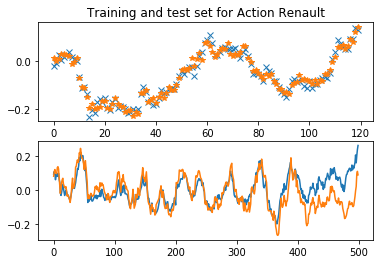
\includegraphics[width=.9\linewidth, scale=0.2]
	{plot/norma.png}
	\caption{Les données dans la base d'apprentissage}
	\label{fig:Base_A}
	\end{subfigure}%
	\begin{subfigure}{.5\textwidth}
	\centering
	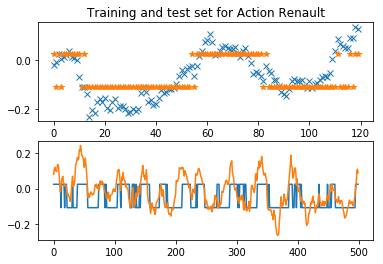
\includegraphics[width=.9\linewidth, scale=0.2]
	{plot/non_norma.png}
	\caption{Les données dans la base de test}
	\label{fig:Base_T}
	\end{subfigure}
\caption{Comparason entre les données non normalisés et normalisés sur les 2 bases}
\label{fig: normalisation}
\end{figure}

\subsubsection{Paramétrage de la base d'apprentissage}

Pour notre projet, il faut aussi faire varier les paramètres différents pour construire la base d'apprentissage, qui sert à tester des différents scénarios.Nous prenons principalement 4 paramètres pour comparer le résultat de chaque scénario : l'horizon, la taille d'apprentissage, la durée du test et le nombre de TIs. Pour lancer des tests sur les différents scénarios, nous faisons chaque fois varier seulement un paramètre afin de trouver la meilleure combinaison de paramètres.\\

Comme nous avons besoin de prédire le rendement dans un horizon, il faut prendre horizon plus de prix pour calculer les derniers rendements dans la base d'apprentissage. Nous avons commencé le test après un décalage de horizon, c'est-à-dire que nous ne pouvons pas utiliser les données just après pour faire le test. Dans notre projet, nous pouvons considérer la période de décalage comme la base de validation. La figure \ref{fig:BA} est une illustration plus claire : \\

\begin{figure}[H]
	\centering
	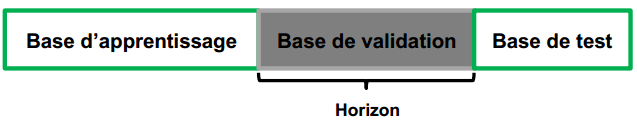
\includegraphics[width=.5\linewidth, scale=0.2]
	{plot/BA.png}
	\caption{La construction de la base}
	\label{fig:BA}
\end{figure}

Nous avons pris tous les 13 TIs au début de notre projet, nous voudrons collecter plus d’informations pour faire la prédiction, nous avons considéré que cette combinaison de TIs est plus robuste. Pour savoir si le nombre de TIs a un impact sur la performance de notre système, nous avons diminué le nombre de TIs et refait des tests avec la dimension réduite en entrée du réseau. Les nombres de TIs que nous avons choisi sont 13, 12 (élimination d'un TI) et 4 (un TI par catégorie).

\subsection{Choix du modèle}

De nombreuses études ont largement admis que la non-linéarité existe sur les marchés financiers et que les réseaux de neurones peuvent être efficacement utilisés pour découvrir cette relation. Les modèles de réseaux de neurones pour l'estimation sont ensuite examinés pour leur capacité à fournir une prévision efficace des valeurs futures.\\

Nous avons utilisé l'algorithme de perceptron multicouche à rétropropagation. Le perceptron multicouche est un type de réseau organisé par plusieurs couches, chaque couche est constituée d'un nombre variable de neurones, les neurones de la dernière couche étant les sorties du système global. Dans notre cas, l'entré de reseau est les TIs et la sortie est le rendement. L'algoritnme de rétropropagation du gradient déscendant est pour minimiser l'erreur afin de converger. Les figures \ref{fig:RN} et \ref{fig:base} représentent la structure de notre réseau de neurones et nos examples d'entrées en format matriciel :\\

\begin{figure}[H]
	\centering
	\begin{subfigure}{.5\textwidth}
	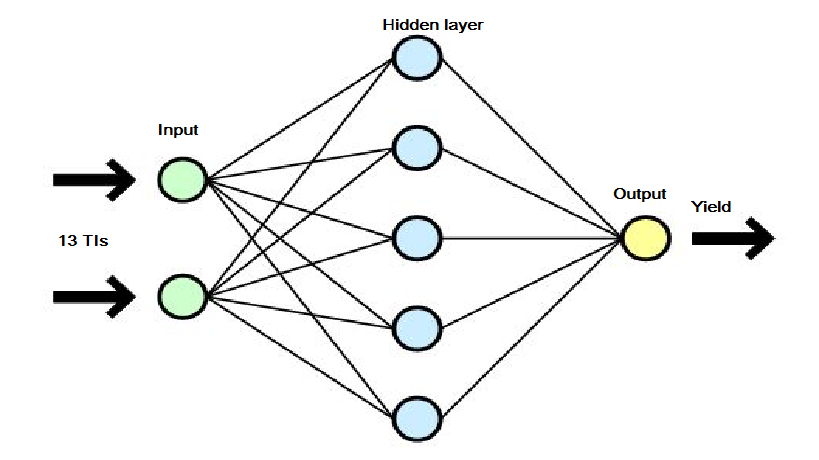
\includegraphics[width=.9\linewidth, scale=0.2]
	{plot/RN.png}
	\caption{La structure de réseaux neurones}
	\label{fig:RN}
	\end{subfigure}%
	\begin{subfigure}{.5\textwidth}
	\centering
	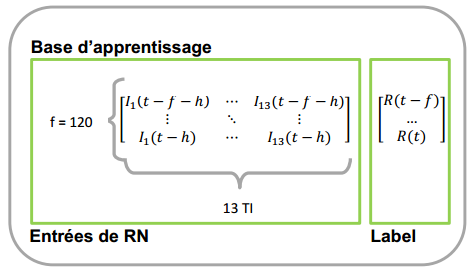
\includegraphics[width=.9\linewidth, scale=0.2]
	{plot/base.png}
	\caption{L'entrée de base d'apprentissage}
	\label{fig:base}
	\end{subfigure}
\caption{L'influence de l'horizon sur en vue global sur 15 ans}
\label{fig:structure_rn}
\end{figure}

Dans le modèle de réseaus neurones, nous avons besoin de choisir le nombre de neurones, le nombre de couches cachés, le taux d'apprentissage, la fonction d’activation et le nombre d'itération. Dans notre projet, nous avons pris une seule couche cachée avec 25 neurones et nous avons paramétré le taux d'apprentissage initial égale à 0,1. Nous avons pris la fonction sigmoid $ f(x) = \frac{1}{1 + exp^{-x}} $ comme la fonction d'activation et notre nombre d'itération est 80000.

\subsection{Préparation des scénarios}

Pour lancer les simulations différentes, nous n'avons changé qu'un seul indicateur dans chaque scénario de test. Comme nous avons dit avant, il y a 4 paramètres pour construire notre base d'apprentissage. Nous avons préparé les scénarios en variant sur un des indicateurs pour choisir une valeur plus favorable pour chaque paramètre. \\

En général, la contrainte de la prédiction d'une série temporelle est la non stationnalité de données, nous ne pouvons pas utiliser les données non corrélées pour faire la prédiction, donc il faut bien défini la durée d'apprentissage. Par conséquent, nous avons besoin de savoir le nombre de patternes à apprendre, si nous prenons trop de patternes, il y a un coût d'apprentissage très élevé et aussi il peut produire le problème de sur-apprentissage. Cependant, si nous prenons pas assez de patternes, la base ne peut pas générer la bonne prédiction, parce qu'elle n'a pas assez d'examples à s'entraîner. \\

Pour savoir la féquence de la gestion de portefeuille, il faut varier sur l'horizon de rendement. Le mouvement du marché est plus petit pendant un horizon plus court, mais dans la réalité nous ne pouvons pas relancer un portefeuille très fréquemment. Par contre, si nous utilisons un horizon plus long, il y a un risque d'avoir une performance très mauvaise. \\

La base de test est pour vérifier le résultat de l'apprentissage et aussi pour mesurer la performance de prédiction. Nous varions sur la taille de test pour savoir pendant combien de temps maximum le modèle est toujours valable et s'il y a un recyclage sur les valeurs prédites. \\

Dans un premier temps, nous prenons tout les 13 TIs pour les autres scénarios, mais il faut aussi considérer l'influence du nombre de TIs. Nous allons caluler la corrélation entre les 13 TIs et essayer de réduire la dimension de nombre de TIs. Dans l'article [Stock Picking by Probability–Possibility Approaches], elle propose plusieurs de combinaisons pour les TIs. Les combinaisons plus intéréssantes sont tout les 13 TIs, les 12 TIs (sauf EMA), les 4 TIs (un par catégorie, soit SMA,CCI,BB1,EMV).\\

Dans la partie suivante, nous vous présentons nos résultats par les différents types de scénarios. En parallèle, nous montrons les explications plus raisonables pour mettre un vrai sens à notre projet. Ensuite, nous avons aussi besoin d'évaluer la performance de notre modèle de prédiction.




  





